
\PassOptionsToPackage{dvipsnames}{xcolor}

\documentclass[11pt,twoside,a4paper]{book}

\usepackage{estilos} %Relacionado ao arquivo estilos.sty com os packages usados


\title{Equações de Derivadas Parciais}
\author{MAP0413}
\date{1º semestre de 2019 \\ atualizadas até a aula de ?}

\begin{document}

\maketitle

\tableofcontents

\newpage

\chapter{Introdução}

Vamos ver os tipos mais básicos de equações diferenciais parciais (EDP). Adotaremos a notação $u_x = \frac{\partial u}{\partial x}$ quando conveniente. 

\section{Conceitos iniciais e exemplos}

\subsection{EDP de 1ª ordem em 2 variáveis}

Uma \emph{EDP de 1ª ordem em 2 variáveis} é uma equação do tipo:
\[
f\Bigg(x,y,u,\pd{u}{x},\pd{u}{y}\Bigg) = 0
\]


\smallskip
\noindent
\textbf{Exemplo 1}

\smallskip
\noindent
Consideremos a EDP:
\[
\pd{u}{x}+y\pd{u}{y} = 0
\]
Por exemplo, seja $u(x,y)=f(e^{-x}y)$ (mais tarde mostraremos qual foi a motivação para pensarmos em funções desse tipo), com $f:\mathbb{R}\rightarrow\mathbb{R}$ de classe $\mathcal{C}^1$. Então:
\[
\pd{u}{x}=f'(e^{-x}y)(-ye^{-x})
\]
\[
\pd{u}{y}=f'(e^{-x}y)e^{-x}
\]

\smallskip
\noindent
Assim $u$ é uma solução da equação e temos $u(0,y)=f(y)$. $\square$

\subsection{EDP de 2ª ordem em 2 variáveis}

Uma \emph{EDP de 2ª ordem em 2 variáveis} é uma equação do tipo:
\[
f\Bigg(x,y,u,\pd{u}{x},\pd{u}{y},\pd[2]{u}{x},\md{u}{2}{x}{}{y}{},\pd[2]{u}{y}\Bigg) = 0
\]

\subsection{Equações da Física Matemática}

Vamos mostrar exemplos de EDP's que são importantes para diversas aplicações.

\subsubsection{Equação de Laplace}

\[\Delta u \coloneqq \pd[2]{u}{x} + \pd[2]{u}{y} = 0\]

\noindent
As soluções dessa EDP são conhecidas como \emph{funções harmônicas}. Por exemplo, $u(x,y) = x^3 - 3 xy^2$ é uma função harmônica. (Verifique!)

\noindent
O potencial eletrostático $V(x,y,z).$ numa região onde não existam cargas, verifica a equação:


\[
    \pd[2]{V}{x} + \pd[2]{V}{y} + \pd[2]{V}{z} = 0
\]

\subsubsection{Equação da Onda}

\[
\pd[2]{u}{t} = c^2 \Delta u
\]

\noindent
Uma função de onda, em duas dimensões, é uma função $f(x,y,t)$ solução da equação

\[\pd[2]{f}{t} =  v^2 \Bigg(\pd[2]{f}{x} + \pd[2]{f}{y}\Bigg)
\]

\noindent
onde $v$ é uma constante (velocidade de propagação). Neste caso, existem $3$ variáveis independentes, nomeadamente, as duas coordenadas espaciais $x$ e $y$, e o tempo $t.$

\subsubsection{Equação de Calor}

\[
\pd{u}{t} = k \Delta u, \quad k > 0
\]

\subsubsection{Equação de Burgers}

A \emph{equação de Burgers} modela processos convectivos unidimensionais:

\[
\pd{u}{t} + u \pd{u}{x} = 0
\]

\subsubsection{Equação de Korteweg-de Vries}

A \emph{equação de Korteweg-de Vries}, conhecida também como KdV, é responsável por descrever matematicamente o comportamento de ondas em superfícies de águas rasas.


\[
\pd{u}{t} - 6 u \pd{u}{x} + \pd[3]{u}{x} = 0
\]

\begin{figure}[!ht]
    \centering
    
\includegraphics[width=.40\textwidth]{figuras/onda_cnoidal.png}
    \caption{A onda senoidal é um exemplo de onda periódica que é solução da equação KdV.}
    \label{fig:onda_cnoidal}
\end{figure}


\subsubsection{Superfícies mínimas}

Seja $\Omega \subseteq \mathbb{R}^2$ um aberto, $h \colon \partial \Omega \to \mathbb{R}$ e $u \colon \overline{\Omega} \to \mathbb{R}$, de modo que $u \upharpoonright_{\partial \Omega} = f$.

\noindent
Então, a área da superfície é dada por
\[
A(S) = \int\limits_{\Omega} \sqrt{1 + \left(\frac{\partial^2 u}{\partial x^2}\right)^2 + \left(\frac{\partial^2 u}{\partial y^2}\right)^2} dx dy
\]

\noindent
A função $u(x,y)$ que torna a superfície $S$ minimal satisfaz a seguinte equação diferencial parcial:
\[
\left(1 + \left(\frac{\partial^2 u}{\partial y^2} \right)^2 \frac{\partial^2 u}{\partial x^2} \right) - 2 \frac{\partial u}{\partial x} \cdot \frac{\partial u}{\partial y} \cdot \frac{\partial^2 u}{\partial x \partial y} + \left(1 + \left(\frac{\partial^2 u}{\partial x^2} \right)^2 \frac{\partial^2 u}{\partial y^2} \right) = 0 
\]
\begin{figure}[!ht]
    \centering
    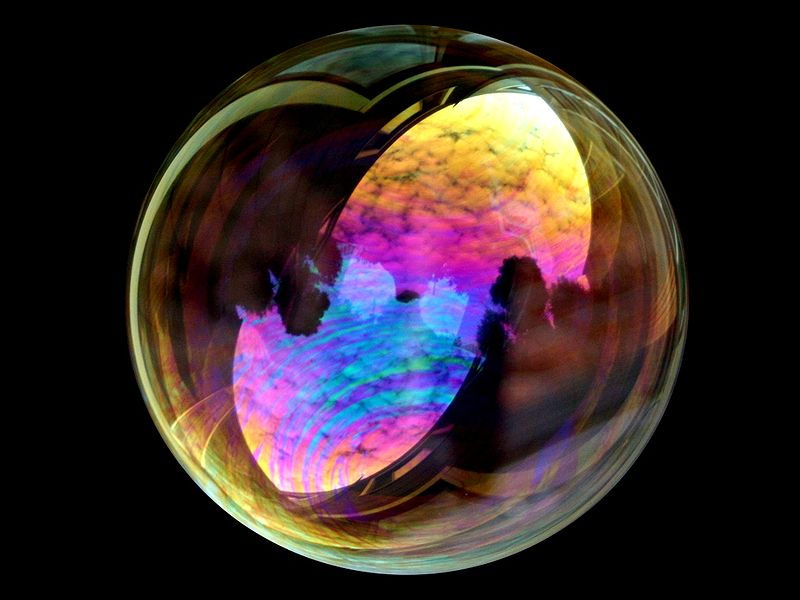
\includegraphics[width=.40\textwidth]{figuras/bolha_sabao.png}
    \caption{A bolha de sabão é um exemplo de superfície minimal.}
    \label{fig:bolha_sabao}
\end{figure}

\newpage

\section{EDP de 1ª ordem em 2 variáveis}

\subsection{Tipos de EDP}

De acordo com sua estrutura, as EDP podem ser classificadas em diversas categorias. As principais são:
\begin{itemize}
    \item[$\clubsuit$] \textbf{Linear}, da forma 
    \[
    a(x,y) \frac{\partial u}{\partial x} + b(x,y) \frac{\partial u}{\partial y} = c(x,y)u
    \]
    \item[$\textcolor{red}{\varheart}$] \textbf{Semilinear}, da forma 
    \[
    a(x,y) \frac{\partial u}{\partial x} + b(x,y) \frac{\partial u}{\partial y} = c(x,y,u)
    \]
\item[$\spadesuit$] \textbf{Quasilinear}, da forma 
    \[
    a(x,y,u) \frac{\partial u}{\partial x} + b(x,y,u) \frac{\partial u}{\partial y} = c(x,y,u)
    \]
    
 \item[$\textcolor{red}{\vardiamond}$] \textbf{Não-linear}, como a equação KdV.
\end{itemize}

\subsection{EDPs lineares homogêneas}

Agora consideraremos a EDP do tipo (1):
\begin{equation*}
    a(x,y) \frac{\partial u}{\partial x} + b(x,y) \frac{\partial u}{\partial y} = 0
\end{equation*}

\smallskip
\noindent
Dados:

\begin{enumerate}
    \item[$\bullet$] Uma função $u$ de um aberto $\Omega\subseteq\mathbb{R}^2$ em $\mathbb{R}$ de classe $\mathcal{C}^1$
    \item[$\bullet$] Uma curva parametrizada $\gamma(s)=(x(s),y(s))$ de um aberto $I\subseteq\mathbb{R}$ em $\Omega$ de classe $\mathcal{C}^1$
\end{enumerate}

\smallskip
\noindent
Então, pela regra da cadeia, temos:

\begin{equation*}
    (u\circ\gamma)'(s)=x'(s) u_x(\gamma(s))+y'(s) u_y(\gamma(s))
\end{equation*}

\smallskip
\noindent
Assim, seria interessante encontrarmos curvas parametrizadas do tipo $\gamma(s)=(x(s),y(s))$ de classe $\mathcal{C}^1$ tais que:

\begin{equation*}
    \begin{cases}
    x'(s)=a(x(s),y(s))       \\
    y'(s)=b(x(s),y(s))      
    \end{cases}
\end{equation*}

\smallskip
\noindent
Chamamos uma curva assim de \textbf{curva característica de (1)}.

\medskip
\noindent
Notemos que, se $u$ é uma solução de (1), então, para toda curva característica $\gamma$, a função $u\circ\gamma$ é constante. De fato temos algo melhor:

\medskip
\noindent
\textbf{Teorema:}

\noindent
\textit{Uma função $u$ de classe $\mathcal{C}^1$ é uma solução de} (1) \textit{se e somente se é constante ao longo de cada curva característica.}

\smallskip
\noindent
\textit{Demonstração:}

\noindent
Se $u$ é constante ao longo das curvas características, então para todo $p\in\Omega$, pelo teorema da existência de soluções de EDOs, existe uma curva característica $\gamma(s)$ tal que $\gamma(0)=p$, assim temos $(u\circ\gamma)'(0)=0$, aí $a(p)u_x(p)+b(p)u_y(p)=0$; logo $u$ é solução de (1). $\square$

\bigskip
\noindent
\textbf{Exemplo 1}

\smallskip
\noindent
\textit{Resolver:}
\begin{equation*}
    u_x+yu_y=0
\end{equation*}

\smallskip
\noindent
\textit{Resolução:}

\smallskip
\noindent
A equação da curva característica $\gamma$ é:
\begin{equation*}
    \begin{cases}
    x'(s)=1       \\
    y'(s)=y(s)     
    \end{cases}
\end{equation*}

\smallskip
\noindent
Para cada $p=(x_0,y_0)$, então a curva $\gamma$ dada por:
\begin{equation*}
    \begin{cases}
    x(s)=s+x_0       \\
    y(s)=y_0e^{s}      
    \end{cases}
\end{equation*}
é uma curva característica tal que $\gamma(0)=p$, aí $u(x_0,y_0)=u(\gamma(0))=u(\gamma(-x_0))=u(0,y_0e^{-x_0})$.

\smallskip
\noindent
Portanto, sendo $f(r)=u(0,r)$, então, para todo ponto $(x,y)$ temos $u(x,y)=f(ye^{-x})$. $\square$

\bigskip
\noindent
\textbf{Exemplo 2}

\smallskip
\noindent
\textit{Resolver:}
\begin{equation*}
    yu_x-xu_y=0
\end{equation*}

\smallskip
\noindent
\textit{Resolução:}

\smallskip
\noindent
A equação da curva característica $\gamma$ é:
\begin{equation*}
    \begin{cases}
    x'(s)=-y(s)       \\
    y'(s)=x(s)     
    \end{cases}
\end{equation*}

\smallskip
\noindent
Para cada $p=(x_0,y_0)$, seja $r=\sqrt{x_0^2+y_0^2}$, então a curva $\gamma$ dada por:
\begin{equation*}
    \begin{cases}
    x(s)=r\cos s       \\
    y(s)=r\sin s      
    \end{cases}
\end{equation*}
é uma curva característica tal que, $\gamma(c)=p$ para algum $c$, aí $u(p)=u(r\cos c,r\sin c)=u(r\cos 0,r\sin 0)=u(r,0)$, aí $u(x_0,y_0)=u\left(\sqrt{x_0^2+y_0^2},0\right)$.

\medskip
\noindent
Logo, sendo $h(r)=u(r,0)$, então para todo ponto $(x,y)$ temos $u(x,y)=h\left(\sqrt{x^2+y^2}\right)$. $\square$

\bigskip
\noindent
Agora estudaremos o chamado \textbf{problema de Cauchy}:

\smallskip
\noindent
\textit{Dados:}
\begin{enumerate}
    \item[$\bullet$] \textit{Curva parametrizada $\Gamma(r)=(\alpha(r),\beta(r))$ de classe $\mathcal{C}^1$.}
    \item[$\bullet$] \textit{Função $h$ de classe $\mathcal{C}^1$.}
\end{enumerate}

\noindent
\textit{Resolver} (1) \textit{sujeito a $u(\Gamma(r))=h(r)$.}

\bigskip
\noindent
Estudemos alguns exemplos para uma melhor ilustração.

\bigskip
\noindent
\textbf{Exemplo 1}

\smallskip
\noindent
\textit{Dada função $h$ de classe $\mathcal{C}^1$, resolver:}
\begin{equation*}
    u_x=0
\end{equation*}
\textit{Sujeito a:}
\begin{equation*}
    u(r,2r)=h(r)
\end{equation*}

\smallskip
\noindent
\textit{Resolução:}

\noindent
Temos uma instância do problema de Cauchy em que:
\begin{equation*}
    \begin{cases}
    \alpha(r)=r       \\
    \beta(r)=2r      
    \end{cases}
\end{equation*}

\smallskip
\noindent
A equação da curva característica $\gamma$ é:
\begin{equation*}
    \begin{cases}
    x'(s)=1       \\
    y'(s)=0    
    \end{cases}
\end{equation*}

\smallskip
\noindent
Para cada $p=(x_0,y_0)$, então a curva $\gamma$ dada por:
\begin{equation*}
    \begin{cases}
    x(s)=s+x_0       \\
    y(s)=y_0      
    \end{cases}
\end{equation*}
é uma curva característica tal que $\gamma(0)=p$, aí $u(x_0,y_0)=u\left(\gamma(0)\right)=u\left(\gamma\left(\frac{y_0}{2}-x_0\right)\right)=u\left(\frac{y_0}{2},y_0\right)=h\left(\frac{y_0}{2}\right)$.

\medskip
\noindent
Logo para todo $(x,y)$ temos $u(x,y)=h\left(\frac{y}{2}\right)$. $\square$

\bigskip
\noindent
\textbf{Exemplo 2}

\smallskip
\noindent
\textit{Dada função $h$ de classe $\mathcal{C}^1$, resolver:}
\begin{equation*}
    u_x=0
\end{equation*}
\textit{Sujeito a:}
\begin{equation*}
    r>0\Rightarrow u(r,r^2)=h(r)
\end{equation*}


\smallskip
\noindent
\textit{Resolução:}

\noindent
Temos uma instância do problema de Cauchy em que:
\begin{equation*}
    \begin{cases}
    \alpha(r)=r       \\
    \beta(r)=r^2      
    \end{cases}
\end{equation*}

\smallskip
\noindent
A equação da curva característica $\gamma$ é:
\begin{equation*}
    \begin{cases}
    x'(s)=1       \\
    y'(s)=0    
    \end{cases}
\end{equation*}

\smallskip
\noindent
Para cada $p=(x_0,y_0)$ com $y_0>0$, então a curva $\gamma$ dada por:
\begin{equation*}
    \begin{cases}
    x(s)=s+x_0       \\
    y(s)=y_0      
    \end{cases}
\end{equation*}
é uma curva característica tal que $\gamma(0)=p$, aí $u(x_0,y_0)=u\left(\gamma(0)\right)=u\left(\gamma\left(\sqrt{y_0}-x_0\right)\right)=u\left(\sqrt{y_0},y_0\right)=h\left(\sqrt{y_0}\right)$.

\medskip
\noindent
Logo, para todo $(x,y)$ tal que $y>0$, temos $u(x,y)=h\left(\sqrt{y}\right)$. $\square$

\bigskip
\noindent
\textbf{Exemplo 3}

\smallskip
\noindent
\textit{Dada função $h$ de classe $\mathcal{C}^1$, resolver:}
\begin{equation*}
    u_t+cu_x=0
\end{equation*}
\textit{Sujeito a:}
\begin{equation*}
    u(0,x)=h(x)
\end{equation*}

\smallskip
\noindent
\textit{Resolução:}

\noindent
Temos uma instância do problema de Cauchy em que:
\begin{equation*}
    \begin{cases}
    \alpha(r)=0       \\
    \beta(r)=r      
    \end{cases}
\end{equation*}

\smallskip
\noindent
A equação da curva característica $\gamma$ é:
\begin{equation*}
    \begin{cases}
    x'(s)=1       \\
    y'(s)=c     
    \end{cases}
\end{equation*}

\smallskip
\noindent
Para cada $p=(t_0,x_0)$, então a curva $\gamma$ dada por:
\begin{equation*}
    \begin{cases}
    x(s)=s+t_0       \\
    y(s)=cs+x_0      
    \end{cases}
\end{equation*}
é uma curva característica tal que $\gamma(0)=p$, assim temos $u(t_0,x_0)=u(\gamma(0))=u\left(\gamma(-t_0)\right)=u(0,-ct_0+x_0)=h(-ct_0+x_0)$.

\medskip
\noindent
Logo para todo $(t,x)$ temos $u(t,x)=h\left(-ct+x\right)$. $\square$

\bigskip
\noindent
É claro que, em cada exemplo, há um abismo entre encontrar uma solução para o problema de Cauchy e saber se não há soluções diferentes. Aliás, um mesmo problema de Cauchy pode ter soluções diferentes (\textcolor{red}{por favor, alguém dê um exemplo disso!}). Não obstante, há condições suficientes para que tenhamos unicidade na solução.

\bigskip
\noindent
Consideremos novamente o problema de Cauchy:

\smallskip
\noindent
\textit{Dados:}
\begin{enumerate}
    \item[$\bullet$] \textit{Curva parametrizada $\Gamma(r)=(\alpha(r),\beta(r))$ de classe $\mathcal{C}^1$.}
    \item[$\bullet$] \textit{Função $h$ de classe $\mathcal{C}^1$.}
\end{enumerate}

\noindent
\textit{Resolver} (1) \textit{sujeito a $u(\Gamma(r))=h(r)$.}

\bigskip
\noindent
Dado $r_0\in I$, sendo $\Gamma(r_0)=(x_0,y_0)$, dizemos que o problema é \textbf{não característico em $r_0$} se e só se tivermos o seguinte:
\begin{equation*}
    \det
    \begin{pmatrix}
    \alpha'(r_0)&a(x_0,y_0)\\\beta'(r_0)&b(x_0,y_0)
    \end{pmatrix}
    \neq 0
\end{equation*}

\smallskip
\noindent
Essa condição quer dizer que a curva de condições iniciais não tangenciará curva característica alguma que passe por $(x_0,y_0)$.

\bigskip
\noindent
\textbf{Teorema da existência e unicidade local para problemas não característicos:}

\noindent
\textit{Se o problema de Cauchy é não característico em $r_0\in I$, então existe uma vizinhança aberta $V$ de $\Gamma(r_0)=(x_0,y_0)$ na qual exista uma única solução definida em $V$.}

\smallskip
\noindent
\textit{Demonstração:}

\noindent
Consideremos a equação característica:

\begin{equation*}
    \begin{cases}
    x'(s)=a(x(s),y(s)) \\
    y'(s)=b(x(s),y(s))
    \end{cases}
\end{equation*}

\smallskip
\noindent
Para $r$, pelo teorema da existência de soluções em EDO, existe uma curva característica $\gamma_r(s)=(X_r(s),Y_r(s))$ tal que $\gamma_r(0)=\Gamma(r)$.

\smallskip
\noindent
Por um abuso de notação, consideremos $\gamma(r,s)=(X(r,s),Y(r,s))=(X_r(s),Y_r(s))$. Pelo teorema da dependência diferenciável de parâmetros iniciais, então $\gamma$ é função de classe $\mathcal{C}^1$.


\smallskip
\noindent
Por hipótese $\left(X\left(r_0,0\right),Y\left(r_0,0\right)\right)=(x_0,y_0)$, assim:
\[
\pd{X}{r}(r_0,0)=\alpha'(r_0),\quad \pd{X}{s}(r_0,0)=a(x_0,y_0)
\]
\[
\pd{Y}{r}(r_0,0)=\beta'(r_0),\quad \pd{Y}{s}(r_0,0)=b(x_0,y_0)
\]

\noindent
Por hipótese, o determinante da matriz é diferente de $0$, assim, pelo teorema da função inversa, existem vizinhança aberta $V$ de $(x_0,y_0)$ e funções $R,S:V\rightarrow\mathbb{R}$ tais que a função $p\mapsto(R(p),S(p))$ seja inversa de $\gamma\upharpoonright_V$.

\smallskip
\noindent
Seja $u(p)=h(R(p))$. Para $r$, então para $s$ temos $u(\gamma_r(s))=h(R(\gamma_r(s)))=h(r)$; em particular $u(\Gamma(r))=u(\gamma_r(0))=h(r)$; logo $u$ é uma solução do problema de Cauchy.

\smallskip
\noindent
Se $v$ fosse outra solução do problema de Cauchy, então para $p\in V$ teríamos $v(p)=v(\gamma_{R(p)}(S(p)))=v(\gamma_{R(p)}(0))=h(R(p))=u(p)$; logo $v=u$. $\square$

\subsection{EDPs semilineares}

Agora consideraremos a EDP do tipo (2):
\begin{equation*}
    a(x,y)\frac{\partial u}{\partial x}+b(x,y)\frac{\partial u}{\partial y}=c(x,y,u)
\end{equation*}

\medskip
\noindent
Por enquanto nos contentaremos em resolver um exemplo:

\bigskip
\noindent
\textbf{Exemplo}

\bigskip
\noindent
\textit{Resolver:}
\begin{equation*}
    \frac{\partial u}{\partial t}+x\frac{\partial u}{\partial x}=u^3
\end{equation*}
\textit{Sujeito a:}
\begin{equation*}
    u(0,x)=\sin x
\end{equation*}

\smallskip
\noindent
\textit{Resolução:}

\noindent
A equação da curva característica é:
\begin{equation*}
    \begin{cases}
    t'(s)=1 \\
    x'(s)=x(s)
    \end{cases}
\end{equation*}

\noindent
Para $p=(t_0,x_0)$, então a curva dada por:
\begin{equation*}
    \begin{cases}
    t(s)=s \\
    x(s)=x_0e^{s-t_0}
    \end{cases}
\end{equation*}
é uma curva característica tal que $\gamma(t_0)=p$.

\smallskip
\noindent
Agora seja $z(s)=u(\gamma(s))$. Então temos o seguinte:

\begin{equation*}
    \begin{cases}
    z'(s)=(z(s))^3 \\
    z(0)=\sin(x_0e^{-t_0})
    \end{cases}
\end{equation*}

\smallskip
\noindent
Nesse caso temos $(z(s))^{-3}z'(s)=1$, aí $\frac{(z(s))^{-2}}{-2}-\frac{(z(0))^{-2}}{-2}=s$, aí $(z(s))^{-2}=(z(0))^{-2}-2s=\frac{1-2s(z(0))^2}{(z(0))^2}$, aí $z(s)=\frac{z(0)}{\sqrt{1-2s(z(0))^2}}=\frac{\sin(x_0e^{-t_0})}{\sqrt{1-2s\sin^2(x_0e^{-t_0})}}$, portanto $u(t_0,x_0)=z(t_0)=\frac{\sin(x_0e^{-t_0})}{\sqrt{1-2t_0\sin^2(x_0e^{-t_0})}}$.

\medskip
\noindent
Logo a solução desejada é $u(t,x)=\frac{\sin(xe^{-t})}{\sqrt{1-2t\sin^2(xe^{-t})}}$. $\square$

\medskip
\noindent
\textit{Pergunta:}

\smallskip
\noindent
Qual é o menor valor de $t>0$ tal que $u$ explode? Em quais $x$?

\smallskip
\noindent
\textit{Resposta:}

\smallskip
\noindent
O menor valor é $t=\frac{1}{2}$, e nesse caso $u$ explode em $x=\frac{\pi}{2}\sqrt{e}$. $\square$


\subsection{EDPs quasilineares}

Agora consideraremos a EDP do tipo (3):
\begin{equation*}
    a(x,y,u)\frac{\partial u}{\partial x}+b(x,y,u)\frac{\partial u}{\partial y}=c(x,y,u),
\end{equation*}
onde $a,b$ e $c$ são funções de classe $\mathcal{C}^1.$ 

\bigskip
\noindent
Em geral, uma EDP é \emph{quasilinear} quando os termos que envolvem as derivadas mais altas são quasilineares.

\bigskip
\noindent
Para função $u$ seja $S_u$ a superfície de equação $u(x,y)-z=0$, e portanto tem um campo normal $(u_x(x,y),u_y(x,y),-1)$. Então, $u$ é solução de (3) se e só se seu campo normal é normal a $(a(x,y,u(x,y)),b(x,y,u(x,y)),c(x,y,u(x,y)))$, e isto ocorre se e só se $S_u$ é tangente ao campo $(a(x,y,u(x,y)),b(x,y,u(x,y)),c(x,y,u(x,y)))$.

\begin{definicao}
As \emph{curvas características} da EDP são as soluções do sistema
\begin{equation*}
    \begin{cases}
    x'(s) = a(x,y,z) \\
    y'(s) = b(x,y,z) \\
    z'(s) = c(x,y,z) \\
    \end{cases}
\end{equation*}
\end{definicao}
\begin{teorema}
Seja $(a(x,y,z),b(x,y,z),c(x,y,z))$ um campo de classe $\mathcal{C}^1$ num aberto $A\subseteq\mathbb{R}^3$. Seja $u(x,y)$ uma função de classe $\mathcal{C}^1$ num aberto $\Omega\subseteq\mathbb{R}^2$ tal que $u[\Omega]\subseteq A$. Se $(a(x,y,u(x,y)),b(x,y,u(x,y)),c(x,y,u(x,y)))$ é tangente a $S_u$ e $(x_0,y_0,z_0)\in S_u$, então a órbita do campo $(x(s),y(s),z(s))$ que passa por $(x_0,y_0,z_0)$ em $s=0$ está contida em $S_u$.
\end{teorema}
\begin{proof}[Demonstração]
Pelo teorema de existência de soluções de EDO, existe uma curva $\gamma(s)=(x(s),y(s),z(s))$ de classe $\mathcal{C}^1$ tal que $\gamma(0)=(x_0,y_0,z_0)$ e:

\begin{equation*}
    \begin{cases}
    x'(s)=a(x(s),y(s),z(s)) \\
    y'(s)=b(x(s),y(s),z(s)) \\
    z'(s)=c(x(s),y(s),z(s)) \\
    \end{cases}
\end{equation*}

\noindent
Definamos a função:

\begin{equation*}
U(s)=z\left(s\right)-u\left(x\left(s\right),y\left(s\right)\right)
\end{equation*}

\noindent
e a função:

\[
\begin{array}{ccc}
G(s,r) & = & c\left(x\left(s\right),y\left(s\right),r+u\left(x\left(s\right),y\left(s\right)\right)\right)\\
 & & -u_x\left(x\left(s\right),y\left(s\right)\right)a\left(x\left(s\right),y\left(s\right),r+u\left(x\left(s\right),y\left(s\right)\right)\right)\\
 & & -u_y\left(x\left(s\right),y\left(s\right)\right)b\left(x\left(s\right),y\left(s\right),r+u\left(x\left(s\right),y\left(s\right)\right)\right)
\end{array}
\]

\noindent
É fácil ver que:

\begin{equation*}
\begin{cases}
U'(s)=G(s,U(s)) \\
U(0)=0
\end{cases}
\end{equation*}

\noindent
além disso, como $u$ satisfaz (3), então:

\begin{equation*}
\begin{cases}
\textbf{0}'(s)=G(s,\textbf{0}(s)) \\
\textbf{0}(0)=0
\end{cases}
\end{equation*}

\noindent
Assim, pelo teorema da unicidade de soluções de EDO, temos $U=\textbf{0}$, ou seja, a órbita $\gamma$ tem sua imagem contida em $S$.

\end{proof}

\begin{teorema}
Uma função $u(x,y)$ de classe $\mathcal{C}^1$ é solução de (3) se e só se a superfície $S_u$ dada pela equação $z=u(x,y)$ é uma reunião disjunta de curvas características.
\end{teorema}
\begin{proof}

Suponha que $S_u$ seja reunião disjunta de curvas características. Para um ponto $(x_0,y_0,z_0)\in S_u$, seja $\gamma(s)=(x(s),y(s),z(s))$ a órbita que passe por $(x_0,y_0,z_0)$ em $s=0$, então a imagem da órbita está contida em $S_u$, assim $\gamma'(s)$ é tangente a $S_u$, ou seja, $(a(x(s),y(s),u(x(s),y(s))),b(x(s),y(s),u(x(s),y(s))),c(x(s),y(s),u(x(s),y(s))))$ é tangente a $S_u$, de modo que $u$ é solução de (3).

\smallskip
\noindent
Suponha que $u$ seja solução de (3), então $(a(x,y,u(x,y)),b(x,y,u(x,y)),c(x,y,u(x,y)))$ é tangente a $S_u$, de modo que, pelo teorema anterior, $S_u$ é reunião disjunta de curvas características.

\end{proof}

\noindent
Agora estudaremos o chamado \textbf{problema de Cauchy quasilinear}:

\smallskip
\noindent
\textit{Dados:}
\begin{enumerate}
    \item[$\bullet$] \textit{Curva parametrizada $\Gamma(r)=(\alpha(r),\beta(r))$ de classe $\mathcal{C}^1$.}
    \item[$\bullet$] \textit{Função $h$ de classe $\mathcal{C}^1$.}
\end{enumerate}

\noindent
\textit{Resolver} (3) \textit{sujeito a $u(\Gamma(r))=h(r)$.}


\bigskip
\noindent
Dado $r_0\in I$, sendo $\Gamma(r_0)=(x_0,y_0)$, dizemos que o problema é \textbf{não característico em $r_0$} se e só se tivermos o seguinte:
\begin{equation*}
    \det
    \begin{pmatrix}
    \alpha'(r_0)&a(x_0,y_0,h(r_0))\\\beta'(r_0)&b(x_0,y_0,h(r_0))
    \end{pmatrix}
    \neq 0
\end{equation*}

\smallskip
\noindent
Essa condição quer dizer que a curva de condições iniciais não tangenciará curva característica alguma que passe por $(x_0,y_0)$.

\bigskip
\noindent
\textbf{Teorema da existência e unicidade local para problemas não característicos:}

\noindent
\textit{Se o problema de Cauchy é não característico em $r_0\in I$, então existe uma vizinhança aberta $V$ de $\Gamma(r_0)=(x_0,y_0)$ na qual exista uma única solução definida em $V$.}

\smallskip
\noindent
\textit{Demonstração:}

\noindent
Consideremos a equação característica:

\begin{equation*}
    \begin{cases}
    x'(s)=a(x(s),y(s),z(s)) \\
    y'(s)=b(x(s),y(s),z(s)) \\
    z'(s)=c(x(s),y(s),z(s))
    \end{cases}
\end{equation*}

\smallskip
\noindent
Para $r$, pelo teorema da existência de soluções em EDO, existe uma curva característica $\gamma_r(s)=(X_r(s),Y_r(s),Z_r(s))$ tal que $\gamma_r(0)=(\Gamma(r),h(r))$.

\smallskip
\noindent
Por um abuso de notação, seja $\gamma(r,s)=(X(r,s),Y(r,s),Z(r,s))=(X_r(s),Y_r(s),Z_r(s))$. Pelo teorema da dependência diferenciável de parâmetros iniciais, $\gamma$ é de classe $\mathcal{C}^1$.


\smallskip
\noindent
Por hipótese $\left(X\left(r_0,0\right),Y\left(r_0,0\right),Z\left(r_0,0\right)\right)=(x_0,y_0,h(r_0))$, assim:
\[
\pd{X}{r}(r_0,0)=\alpha'(r_0),\quad \pd{X}{s}(r_0,0)=a(x_0,y_0,h(r_0))
\]
\[
\pd{Y}{r}(r_0,0)=\beta'(r_0),\quad \pd{Y}{s}(r_0,0)=b(x_0,y_0,h(r_0))
\]

\noindent
Por hipótese, o determinante da matriz é diferente de $0$, assim, pelo teorema da função inversa, existem vizinhança aberta $V$ de $(x_0,y_0)$ e funções $R,S:V\rightarrow\mathbb{R}$ tais que a função $p\mapsto(R(p),S(p))$ seja inversa da função $(r,s)\mapsto(X(r,s),Y(r,s))$.

\smallskip
\noindent
Seja $u(p)=Z(R(p),S(p))$. Para $r$, então $\forall s:u(X_r(s),Y_r(s))=u(X(r,s),Y(r,s))=Z(r,s)=Z_r(s)$; em particular $u(\Gamma(r))=u(X_r(0),Y_r(0))=Z_r(0)=h(r)$; logo $u$ é uma solução do problema de Cauchy.

\smallskip
\noindent
Se $v$ fosse outra solução do problema de Cauchy, então para $p\in V$ teríamos $v(p)=v(X_{R(p)}(S(p)),Y_{R(p)}(S(p)))=Z_{R(p)}(S(p))=u(p)$; logo $v=u$. $\square$

\bigskip
\noindent
\textbf{Exemplo: Equação de Burgers}

\bigskip
\noindent
Consideremos a equação:
\begin{equation*}
    \pd{u}{t}+u\pd{u}{x}=0
\end{equation*}
Sujeito a:
\begin{equation*}
    u(0,x)=f(x)
\end{equation*}
A equação de Burger é um caso de EDP quasilinear.

\smallskip
\noindent
Encontraremos as soluções que estão sob a curva $\Gamma(r) = (0,r)$ tais que $u(\Gamma(r)) = f(r).$

\smallskip
\noindent
Vamos buscar as curvas características $t(r,s), x(r,s), z(r,s):$
\[
    \left\{\begin{array}{ccc}
    t_r'(s) & = & 1 \\
    x_r'(s) & = & z_r(s) \\
    z_r'(s) & = & 0 \\
    \end{array}\right.
\]
Além dessas condições, temos também que 
\[
t_r(0) = \alpha(r) = 0, \quad x_r(0) = \beta(r) = r, \quad z_r(0) = f(r)
\]
Assim:
\[
\left\{
\begin{array}{ccccc}
    t_r'(s) = 1 & , & t_r(0) = 0 & \Rightarrow & t_r(s) = s\\
    x_r'(s) = z(s) & , & x_r(0) = r & \Rightarrow & x_r(s) = sf(r) + r \\
    z_r'(s) = 0 & , & z_r(0) = f(r) & \Rightarrow & z_r(s) = f(r) \\
\end{array}
\right.
\]

\noindent
Precisamos inverter $(t,x)$ com $(r,s)$, ou seja, determinar $R$ e $S$. Como $t(r,s)=s$ e $x(r,s)=sf(r)+r$, então devemos ter $S(t,x)=t$. A determinação de $R$ depende de $f$, pois $r$ está no escopo de $f$.

\smallskip
\noindent
Se $t=0$, então $R(t,x)=x$. Se $t\neq 0$ e $u$ é solução da EDP, então temos $u(t,x)=z(R(t,x),S(t,x))=f(R(t,x))$, aí, como $z(r,s)=sf(r)+r$, então temos $R(t,x)=x-S(t,x)f(R(t,x))=x-tf(R(t,x))=x-tu(t,x)$, assim $u(t,x)=f(x-tu(t,x))$. $\square$

\section{Equação da onda unidimensional}

\subsection{Introdução}

Do ponto de vista físico, a equação de onda unidimensional é responsável por descrever o comportamento e pequenas oscilações em uma corda\footnote{Entende-se um fio fino e flexível.}. Supondo que, em estado de equilíbrio, a corda coincida com o eixo $x$, é possível modelar por meio de EDPs o caso de pequenas oscilações transversais. Por transversal designa-se a oscilação que se realiza em um plano que contém o eixo $x$ e no qual cada elemento da corda se desloca perpendicularmente eixo $x$. Representaremos por $u(x,t)$ o deslocamento transversal de cada ponto $x$ da corda no instante $t$ a partir da sua posição de equilíbrio.
A partir do caso inicial, podemos também generalizar o problema para a situação $n$-dimensional.

\medskip
\noindent
Assim, tomando $n = 1$, temos $u(t,x);$ para $n = 2,$ $u(t,x,y);$ $n = 3, u(t,x,y,z);$ e assim por diante.

\medskip
\noindent
A \emph{equação da onda} é dada por
\begin{equation}\label{eouni}
   \pd[2]{u}{t} = c^2 \Delta u 
\end{equation}

\subsection{Equação genérica da onda unidimensional}

\noindent
Vamos estudá-la particularmente para o caso $n = 1.$ Nessa situação, a equação \ref{eouni} se reduz ao seguinte:
\[
\pd[2]{u}{t} = c^2\pd[2]{u}{x}
\]

\noindent
Relembramos a solução da equação do transporte:
\[
\pd{u}{t}\mp c\pd{u}{x}=0\Rightarrow u(t,x)=f(x\pm ct)
\]

\medskip
\noindent
Note que:
\[
\pd[2]{u}{t}-c^2\pd[2]{u}{x}=0\Rightarrow\left(\pd{}{t}-c\pd{}{x}\right)\left(\pd{}{t}+c\pd{}{x}\right)u
\]

\noindent
e logo $u(x,t)=F(x\pm ct)$ é solução para qualquer $F$ qualquer de classe $\mathcal{C}^2$.

\smallskip
\noindent
Desse modo, se $F,G$ são de classe $\mathcal{C}^2$, então $u(t,x)=F(x+ct)+G(x-ct)$ é solução.

\smallskip
\noindent
Será que todas as soluções podem ser expressas dessa forma?

\begin{proposicao}
Considere a equação da onda 
\[
\pd[2]{u}{t} = c^2 \pd[2]{u}{x}
\]
Então, existem $F, G \colon \mathbb{R} \to \mathbb{R}$ tal que para quaisquer $t,x$ tenhamos:
\[
u(t,x) = F(x + ct) + G(x - ct)
\]

\end{proposicao}
\begin{proof}
Seja $v(r,s)=u\left(\frac{r-s}{2c},\frac{r+s}{2}\right)$. Então: \[
v_s(r,s)=-\frac{1}{2c}u_t\left(\frac{r-s}{2c},\frac{r+s}{2}\right)+\frac{1}{2}u_x\left(\frac{r-s}{2c},\frac{r+s}{2}\right)
\]

\noindent
Assim 

\[
v_{rs}=-\frac{1}{2c}\left(\frac{1}{2c}u_{tt}\left(\frac{r-s}{2c},\frac{r+s}{2})+\frac{1}{2}u_{tx}(\frac{r-s}{2c},\frac{r+s}{2}\right)\right)
\]

\[
+\frac{1}{2}\left(\frac{1}{2c}u_{tx}\left(\frac{r-s}{2c},\frac{r+s}{2}\right)+\frac{1}{2}u_{xx}\left(\frac{r-s}{2c},\frac{r+s}{2}\right)\right)
\]

\[
=-\frac{1}{4c^2}u_{tt}\left(\frac{r-s}{2c},\frac{r+s}{2}\right)+\frac{1}{4}u_{xx}\left(\frac{r-s}{2c},\frac{r+s}{2}\right)=0
\]

\noindent
aí existe $f$ tal que $v_s(r,s)=f(r)$, aí existem $F$ e $G$ tais que $v(r,s)=F(r)+G(s)$, assim $u(t,x)=v(x+ct,x-ct)=F(x+ct)+G(x-ct)$.
\end{proof}

\subsection{Equação da onda unidimensional com condições iniciais}

\noindent
Deseja-se também encontrar soluções de problemas que envolvam a equação da onda que satisfazem certas condições. Como a solução de uma equação da onda depende do tempo $t$, podemos fixar $t = 0,$ estabelecendo uma condição inicial.

\medskip
\noindent
Para isso, vamos estabelecer condições iniciais, o que nos fornecerá um problema de valor inicial (PVI):
\[\begin{array}{cccc}
     \text{Resolver:} & u_{tt} - c^2 u_{xx} & = & 0  \\
     \text{Sujeito a:} & u(0,x) & = & f(x) \\
      & u_t (0,x) & = & g(x)
\end{array}\]

\noindent
Em essência, as funções $f$ e $g$ estão codificando como a corda está no instante inicial e qual sua velocidade, respectivamente.

\smallskip
\noindent
Para esse problema, podemos explicitar a solução, como registrado no seguinte resultado:

\begin{proposicao}
\noindent
Consideremos uma EDP com condições iniciais:
\[\left\{\begin{array}{cc}
     u_{tt} - c^2 u_{xx} = 0  \\
     u(0,x)  = 0 \\
     u_t (0,x) = 0
\end{array}\right.\]
Então: $u(t,x)=0$.
\end{proposicao}
\begin{proof}
Pelo que vimos, existem $F,G$ tais que $u(t,x)=F(x+ct)+G(x-ct)$. Logo $u_t(t,x)=cF'(x+ct)-cG'(x-ct)$, aí temos $0=u(0,x)=F(x)+G(x)$ e $0=u_t(0,x)=cF'(x)-cG'(x)$, assim temos:

\[
\left\{
\begin{array}{ccc}
     0 & = & F'(x)+G'(x) \\
     0 & = & cF'(x)-cG'(x)
\end{array}
\right.
\]

\noindent
Assim temos:

\[
\left\{
\begin{array}{ccc}
     F'(x) & = & \frac{cf'(x)+g(x)}{2c} \\
     G'(x) & = & \frac{cf'(x)-g(x)}{2c}
\end{array}
\right.
\]

\noindent
Portanto:
\[
\left\{
\begin{array}{ccc}
     F(x) & = & \frac{f(x)}{2} + \frac{1}{2c}\int_{0}^xg(s)ds+\delta \\
     G(x) & = & \frac{f(x)}{2} - \frac{1}{2c}\int_{0}^xg(s)ds+\epsilon
\end{array}
\right.
\]

\noindent
Logo $F(x)+G(x)=f(x)+\delta+\epsilon$, mas $f(x)=F(x)+G(x)$, assim $\delta+\epsilon=0$, assim:

\[
u(t,x)=F(x+ct)+G(x-ct)=
\]

\[
=\frac{f(x+ct)}{2} + \frac{1}{2c}\int_{0}^{x+ct}g(s)ds+\delta+\frac{f(x-ct)}{2} - \frac{1}{2c}\int_{0}^{x-ct}g(s)ds+\epsilon
\]

\[
=\frac{f(x+ct)}{2} + \frac{1}{2c}\int_{0}^{x+ct}g(s)ds+\frac{f(x-ct)}{2} - \frac{1}{2c}\int_{0}^{x-ct}g(s)ds
\]

\[
=\frac{f(x+ct)+f(x-ct)}{2} + \frac{1}{2c}\int_{x-ct}^{x+ct}g(s)ds+\epsilon
\]
\end{proof}
\begin{proposicao}

\textbf{(Fórmula de D'Alembert)}

\noindent
Consideremos uma EDP com condições iniciais:
\[\left\{\begin{array}{cc}
     u_{tt} - c^2 u_{xx} = 0  \\
     u(0,x)  =f(x) \\
     u_t (0,x) = g(x)
\end{array}\right.\]
Então:
\[\boxed{u(t,x) = \frac{f(x + ct) + f(x - ct)}{2} + \frac{1}{2c} \int\limits_{x  -ct}^{x + ct} g(s) ds} \]
\end{proposicao}
\begin{proof}
Pelo que vimos, existem $F,G$ tais que $u(t,x)=F(x+ct)+G(x-ct)$. Logo $u_t(t,x)=cF'(x+ct)-cG'(x-ct)$, aí temos $f(x)=u(0,x)=F(x)+G(x)$ e $g(x)=u_t(0,x)=cF'(x)-cG'(x)$, assim temos:

\[
\left\{
\begin{array}{ccc}
     f'(x) & = & F'(x)+G'(x) \\
     g'(x) & = & cF'(x)-cG'(x)
\end{array}
\right.
\]

\noindent
Assim temos:

\[
\left\{
\begin{array}{ccc}
     F'(x) & = & \frac{cf'(x)+g(x)}{2c} \\
     G'(x) & = & \frac{cf'(x)-g(x)}{2c}
\end{array}
\right.
\]

\noindent
Portanto:
\[
\left\{
\begin{array}{ccc}
     F(x) & = & \frac{f(x)}{2} + \frac{1}{2c}\int_{0}^xg(s)ds+\delta \\
     G(x) & = & \frac{f(x)}{2} - \frac{1}{2c}\int_{0}^xg(s)ds+\epsilon
\end{array}
\right.
\]

\noindent
Logo $F(x)+G(x)=f(x)+\delta+\epsilon$, mas $f(x)=F(x)+G(x)$, assim $\delta+\epsilon=0$, assim:

\[
u(t,x)=F(x+ct)+G(x-ct)=
\]

\[
=\frac{f(x+ct)}{2} + \frac{1}{2c}\int_{0}^{x+ct}g(s)ds+\delta+\frac{f(x-ct)}{2} - \frac{1}{2c}\int_{0}^{x-ct}g(s)ds+\epsilon
\]

\[
=\frac{f(x+ct)}{2} + \frac{1}{2c}\int_{0}^{x+ct}g(s)ds+\frac{f(x-ct)}{2} - \frac{1}{2c}\int_{0}^{x-ct}g(s)ds
\]

\[
=\frac{f(x+ct)+f(x-ct)}{2} + \frac{1}{2c}\int_{x-ct}^{x+ct}g(s)ds+\epsilon
\]
\end{proof}

\begin{proposicao}
Consideremos uma EDP com condições iniciais:
\[\left\{\begin{array}{cc}
     u_{tt} - c^2 u_{xx} = 0  \\
     u(0,x)  =f(x) \\
     u_t (0,x) = g(x)
\end{array}\right.\]
Então:
\begin{enumerate}
    \item[a)] Se $f$ e $g$ são ímpares, então $u(t,x)$ é ímpar em $x$.
    \item[b)] Se $f$ e $g$ são pares, então $u(t,x)$ é par em $x$.
\end{enumerate}
\end{proposicao}
\begin{proof}

Consideremos a solução:

\[u(t,x) = \frac{f(x + ct) + f(x - ct)}{2} + \frac{1}{2c} \int\limits_{x  -ct}^{x + ct} g(s) ds \]

\noindent
Para $e\in\mathbb{R}$, se para todo $x\in \mathbb{R}$ temos $f(-x)=ef(x)$ e $g(-x)=eg(x)$, então:

\[
u(t,-x)=\frac{f(-x + ct) + f(-x - ct)}{2} + \frac{1}{2c} \int\limits_{-x  -ct}^{-x + ct} g(s) ds
\]

\[
=\frac{ef(x - ct) + ef(x + ct)}{2} + \frac{1}{2c} \int\limits_{x + ct}^{x - ct} g(-r) (-1) dr
\]

\[
=\frac{ef(x + ct) + ef(x - ct)}{2} - \frac{e}{2c} \int\limits_{x + ct}^{x - ct} g(r) dr
\]

\[
=e\left(\frac{f(x + ct) + f(x - ct)}{2} + \frac{1}{2c} \int\limits_{x - ct}^{x + ct} g(r) dr\right)=eu(t,x)
\]

\end{proof}

\begin{proposicao}

\noindent
\textbf{(Fórmula de Duhamel)}

\noindent
Seja uma EDP com condições iniciais
\[\left\{\begin{array}{l}
     u_{tt} - c^2 u_{xx} = h(t,x)  \\
     u(0,x)  =f(x) \\
     u_t(0,x) = g(x)
\end{array}\right.\]
Então,
\[\boxed{u(t,x) = \frac{f(x + ct) + f(x - ct)}{2} + \frac{1}{2c}\int\limits_{x  -ct}^{x + ct} g(s) ds + \frac{1}{2c} \int\limits_{0}^{t} \left( \int\limits_{x - c(t-s)}^{x + c(t-s)} h(s,y) dy  \right) ds} \]
\end{proposicao}
\begin{proof}

Seja: 
\[
v(t,x)=\frac{1}{2c} \int\limits_{0}^{t} \left( \int\limits_{x - c(t-s)}^{x + c(t-s)} h(s,y) dy  \right) ds
\]



\end{proof}


\begin{definicao}
A \emph{energia} é dada por
\[
E(t) = \frac{1}{2} \int\limits_{-\infty}^\infty \left( \left(   \pd{u}{t}(t,x)\right)^2 + c^2\left(   \pd{u}{x}(t,x)\right)^2 \right) dx
\]
\end{definicao}

\subsection{Equação da onda unidimensional numa corda truncada}

\noindent
Dependendo do tipo de corda que estamos estudando, é necessário também estabelecer condições de contorno.

\medskip
\noindent
Por exemplo, pode ser que queiramos estudar o comportamento de uma corda com uma

\medskip
\noindent
As condições de contorno mais importantes são as de Dirichlet e de Neumann. 

\begin{definicao}\index{condição de Dirichlet}
Considere uma EDP cuja solução seja $u(t,x).$ A \textit{condição de Dirichlet} é dada pelo seguinte:
\[u(t,0) = 0 = u(t,L) 
\]
\end{definicao}
\begin{definicao}\index{condição de Neumann}
Considere uma EDP cuja solução seja $u(t,x).$ A \textit{condição de Neumann} é dada pelo seguinte:
\[\pd{u}{x}(t,0) = 0
\]
\end{definicao}

\noindent
Como exemplo, considere o caso das cordas do violão. A afinação das cordas do violão dependem da temperatura. Podemos considerar
\[
u(t,0) = 0 = u(t,L) 
\]
\[
c^2 = \frac{T}{\mu}
\]
Pela última equação, também conhecida como \emph{Lei de Taylor}, percebe-se que a velocidade $c$ da corda adquirida em determinada oscilação depende da força de tração $T$ e da densidade linear de massa da corda $\mu$. Relembrando conceitos de física, a densidade linear de massa é definida como a razão entre a massa $m$ e o comprimento $\ell$ da corda. Supondo idealmente uma corda de formato cilíndrico, com densidade volumétrica $\rho$, temos que:
\[
\rho = \frac{m}{V} \Rightarrow \rho = \frac{m}{A \cdot \ell} \Rightarrow \textcolor{Verdeest}{\frac{m}{\ell}} = \rho \textcolor{blue}{A} \Rightarrow
\textcolor{Verdeest}{\mu} = \rho \textcolor{blue}{\frac{\pi D^2}{4}}
\]

\noindent
Para resolver este problema, precisamos do \emph{método de separação de variáveis}.
\section{Separação de variáveis}

Consideremos o problema:

\medskip
\noindent
\textit{Resolver a equação:}
\begin{equation*}
    u_{tt}-c^2u_{xx}=0\text{ com $0<x<l$}
\end{equation*}

\noindent
\textit{Sujeito a:}
\begin{equation*}
    u(t,0)=u(t,l)=0
\end{equation*}

\smallskip
\noindent
Consideremos uma função da forma:
\begin{equation*}
    u(t,x)=T(t)\varphi(x)
\end{equation*}
\begin{equation*}
    \varphi(0)=\varphi(l)=0
\end{equation*}
\begin{equation*}
    \varphi\not\equiv 0
\end{equation*}

\noindent
Para satisfazer a equação devemos ter
\begin{equation*}
    T''(t)\varphi(x)=c^2T(t)\varphi''(x)  
\end{equation*}
assim:

\begin{equation*}
    \frac{T^{\prime \prime}(t)}{c^2T(t)}=\frac{\varphi''(x)}{\varphi(x)}=-\lambda
\end{equation*}


\noindent
Concentremo-nos na função $\varphi$, então temos:

\begin{equation*}
    \varphi''(x)+\lambda\varphi(x)=0
\end{equation*}
\begin{equation*}
    \varphi(0)=\varphi(l)=0
\end{equation*}
\begin{equation*}
    \varphi\not\equiv 0
\end{equation*}

\section{Séries de Fourier}

\begin{definicao}


Uma \emph{Série de Fourier} de uma função periódica $f \colon [-L, L] \to \mathbb{R}$ de classe $\mathcal{C}^1$ é uma série infinita da forma
\[f(x) = c_0 + \sum\limits_{n = 1}^\infty a_n \cos(n  x) + \sum\limits_{n = 1}^\infty b_n \sen(n x)\]

\end{definicao}

Cada um dos valores $c_0, a_n, b_n$ podem ser univocamente determinados, como mostra a
\begin{proposicao}\label{coefi}
Os valores $c_0, a_n, b_n$ são conhecidos como \emph{coeficientes de Fourier}, e são dados por
\[
c_0 = \frac{1}{2 L} \int\limits_{-L}^L f(x) \dif {x}
\] e, para todo $n \in \mathbb{N}$
\[
a_n = \frac{1}{L} \int\limits_{- L}^L f(x) \cos(nx) \dif x \quad \mbox{e} \quad  b_n = \frac{1}{L} \int\limits_{- L}^L f(x) \sen(nx) \dif x 
\]
\end{proposicao}
\begin{proof}[Demonstração]
É fácil ver que $c_0 = \frac{1}{2 L} \int\limits_{-L}^L f(x) \dif {x}.$ Para encontrar os valores da sequência $(a_n)_{n \ge 0},$ vamos utilizar que, para $j, k \in \mathbb{N}:$\footnote{Estas relações são chamadas de \emph{relações de ortogonalidade}, por sua ligação com o produto interno definido no intervalo $[a,b]$ por $\langle f, g \rangle = \int\limits_a^b f(x) g(x) \dif x$}
\[
\int\limits_{- L}^L \cos(jx) \cos(kx) \dif x = \int\limits_{- L}^L \cos(jx) \cos(kx) \dif x = L \delta_{jk}
\]
e
\[
\int\limits_{- L}^L \sen(jx) \cos(kx) \dif x = 0
\]
onde $\delta_{jk}$ representa o \emph{Delta de Kronecker}.

Observe que

\[
\int\limits_{-L}^L \textcolor{red}{f(x)} \cos(kx) \dif x = \int\limits_{-L}^L \textcolor{red}{\left(c_0 + \sum\limits_{n = 1}^\infty a_n \cos(n x) + \sum\limits_{n = 1}^\infty b_n \sen(n  x) \right)} \cos(kx) \dif x =
\]
\[\textcolor{red}{c_0} \int\limits_{-L}^L \cos(kx) \dif x + \textcolor{red}{\sum\limits_{n = 1}^\infty a_n \cos(n  x)} \int\limits_{-L}^L \cos(kx) \dif x + \textcolor{red}{ \sum\limits_{n = 1}^\infty b_n \sen(n x)} \int\limits_{-L}^L \cos(kx) \dif x =\]
\[
c_0 \int\limits_{-L}^L \cos(kx) \dif x + \sum\limits_{n = 1}^\infty a_n \underbrace{\int\limits_{-L}^L  \cos(n  x) \cos(kx) \dif x}_{= L a_k} + \sum\limits_{n = 1}^\infty b_n  \underbrace{\int\limits_{-L}^L \sen(n  x) \cos(kx) \dif x}_{=0} \Rightarrow\]
\[\int\limits_{- L}^L f(x) \cos(kx) \dif x = L a_k \Rightarrow \boxed{a_k = \frac{1}{L} \int\limits_{-L}^L f(x) \cos(kx) \dif x }\]
Analogamente, segue o resultado para $b_n.$
\end{proof}


Como exemplo motivador, vamos estudar a Série de Fourier de um sinal periódico digital, que é descrita pela função

\begin{equation}\label{equa}
f(t) = \frac{1}{2} + \frac{2}{\pi} \left( \sum\limits_{n = 0}^\infty \frac{\sen((2n+1) \omega_o t)}{2n+1} \right)
\end{equation}

onde $\omega_0 = 2 \pi f_0,$ para $f_0 = 100 \cdot 8 = 800 \ \mbox{Hz},$ ou seja, $\omega_0 = 1600 \pi \ \mbox{rad/s}.$

Esta função é um caso particular da conhecida \textbf{Square Wave Series} $\sqcap\ \hspace{-7pt}\sqcup (x)$, dada por
\[
\sqcap\ \hspace{-7pt}\sqcup (x) = \sen(x) + \frac{\sen(3x)}{3} + \frac{\sen(5x)}{5} + \frac{\sen(7x)}{7} + \ldots
\]


\subsection{Análise gráfica}

Vamos agora estudar o gráfico de $f(t)$ para observar como esta se comporta.

Primeiramente, pode-se notar que 
\[f(t) = \frac{1}{2} + \lim\limits_{k \to \infty} \frac{2}{\pi} \left( \sum\limits_{n = 0}^{k} \frac{\sen(1600(2n+1) \pi t)}{2n+1} \right),
\]

o que torna interessante observar os gráficos dos primeiros termos da sequência de funções $(f_k)_{k \ge 0},$ onde $f_k(t) = \frac{1}{2} + \frac{2}{\pi} \left( \sum\limits_{n = 0}^{k} \frac{\sen(1600(2n+1) \pi t)}{2n+1} \right)$
Abaixo, temos os gráficos de $f_0(t), f_1(t), f_2(t)$ e $f_4(t):$


\begin{figure}[h]
    \centering
    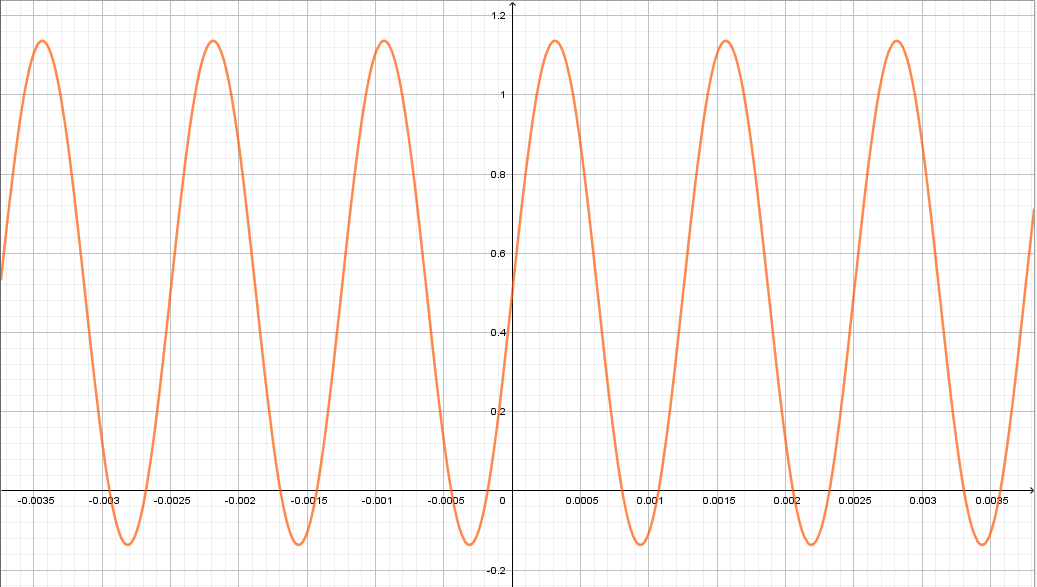
\includegraphics[width=.950\textwidth]{figuras/grafiof0malha.png}
    \caption{Gráfico de $f_0(t) = \frac{1}{2} + \frac{2}{\pi} \left( \sen( 1600 \pi t)  \right)  $}
    \label{fig:1}
\end{figure}

\begin{figure}
    \centering
    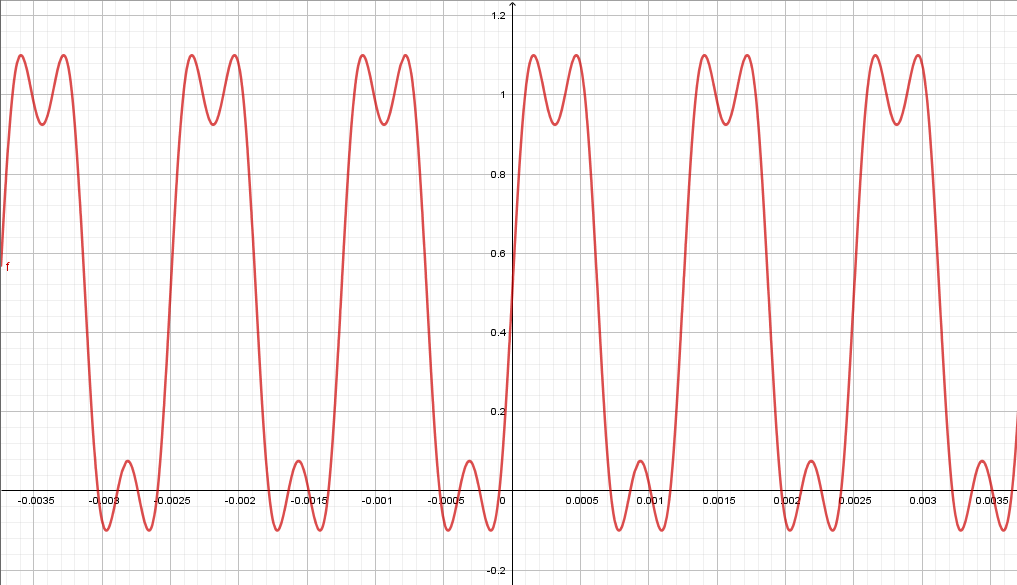
\includegraphics[width=.950\textwidth]{figuras/grafiof1malha.png}
    \caption{Gráfico de $f_1(t) = \frac{1}{2} + \frac{2}{\pi} \left( \sen( 1600 \pi t) + \frac{\sen( 3*1600 \pi t)}{3}  \right)  $}
    \label{fig:2}
\end{figure}


\begin{figure}
    \centering
    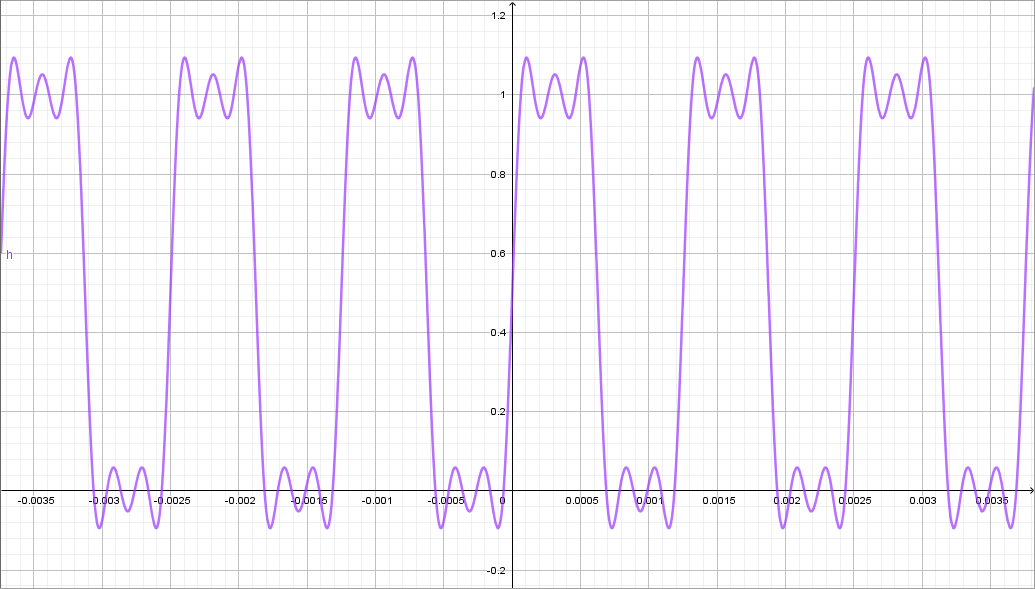
\includegraphics[width=.950\textwidth]{figuras/grafiof2malha.png}
    \caption{Gráfico de $f_2(t) = \frac{1}{2} + \frac{2}{\pi} \left( \sen( 1600 \pi t) + \frac{\sen( 3*1600 \pi t)}{3}   + \frac{\sen( 5*1600 \pi t)}{5} \right)  $}
    \label{fig:3}
\end{figure}


\begin{figure}
    \centering
    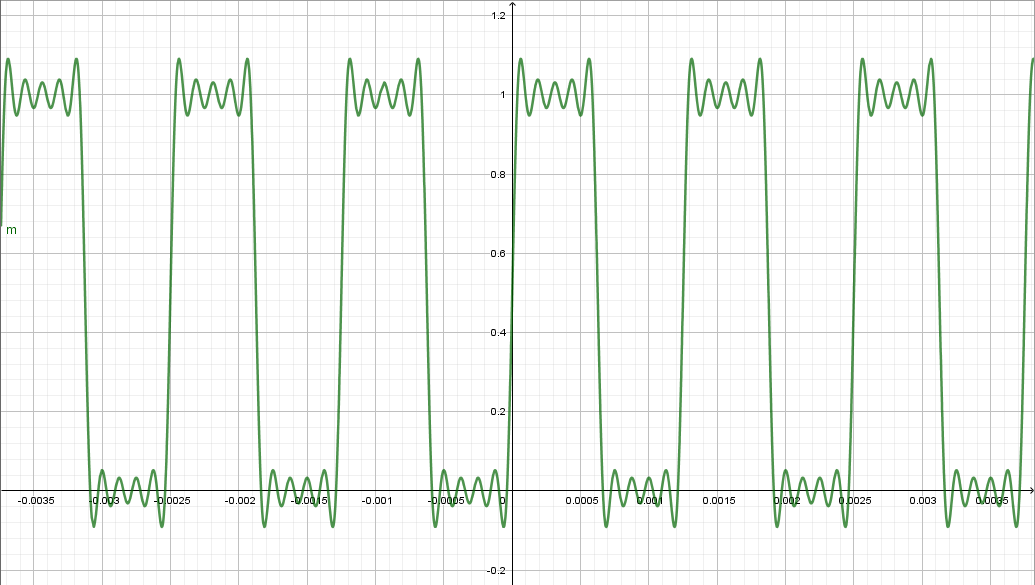
\includegraphics[width=.95\textwidth]{figuras/grafiof4malha.png}
    \caption{Gráfico de $f_4(t) =\frac{1}{2} + \frac{2}{\pi} \left( \sum\limits_{n = 0}^{4} \frac{\sen(1600(2n+1) \pi t)}{2n+1} \right)  $}
    \label{fig:4}
\end{figure}
\newpage
Continuando a plotar os gráficos, veremos que estes tendem a formar padrões constantes, alternando posições em que a função vale $0$ ou $1$. 

De fato, temos que $\lim\limits_{k \to \infty} f_k(t) = f(t), $ onde 
\begin{equation}\label{limite}
f(t) = \left\{\begin{array}{lc}
1, & \mbox{se } t \in \bigcup\limits_{\ell =-\infty}^\infty \left] \frac{2 \ell \pi}{\omega_0}, \frac{(2 \ell + 1) \pi}{\omega_0} \right] \\
0, & \mbox{caso contrário.} 
\end{array} \right.
\end{equation}
Em suma, a função \ref{limite} é uma função alternante, que vale $1$ numa união infinita de intervalos $\ldots \cup \left]  -\frac{4 \pi}{\omega_0}, -\frac{3 \pi}{\omega_0} \right] \cup \left]  -\frac{2 \pi}{\omega_0}, -\frac{ \pi}{\omega_0} \right] \cup \left]  0, \frac{\pi}{\omega_0} \right] \cup \left]  \frac{2 \pi}{\omega_0}, \frac{3 \pi}{\omega_0} \right] \cup \ldots$ e $0$ nos demais pontos. No nosso caso, a função \ref{equa} vale $1$ na união infinita de intervalos $\ldots \cup \left]  -\frac{1}{400}, -\frac{3}{1600} \right] \cup \left]  -\frac{1}{800}, -\frac{1}{1600} \right] \cup \left]  0, \frac{1}{1600} \right] \cup \left]  \frac{1}{800}, \frac{3}{1600} \right] \cup \ldots$. Dessa forma, temos na verdade que
\[
f(t) = \frac{1}{2} + \frac{2}{\pi} \left( \sum\limits_{n = 0}^\infty \frac{\sen((2n+1) \omega_o t)}{2n+1} \right) = \left\{\begin{array}{lc}
1, & \mbox{se } t \in \bigcup\limits_{\ell =-\infty}^\infty \left] \frac{2 \ell \pi}{\omega_0}, \frac{(2 \ell + 1) \pi}{\omega_0} \right] \\
0, & \mbox{caso contrário.} 
\end{array} \right.
\]
A figura \ref{figugraf} mostra o gráfico do sinal digital original que é representado pela equação \ref{equa}:

\begin{figure}[!ht]
    \centering
    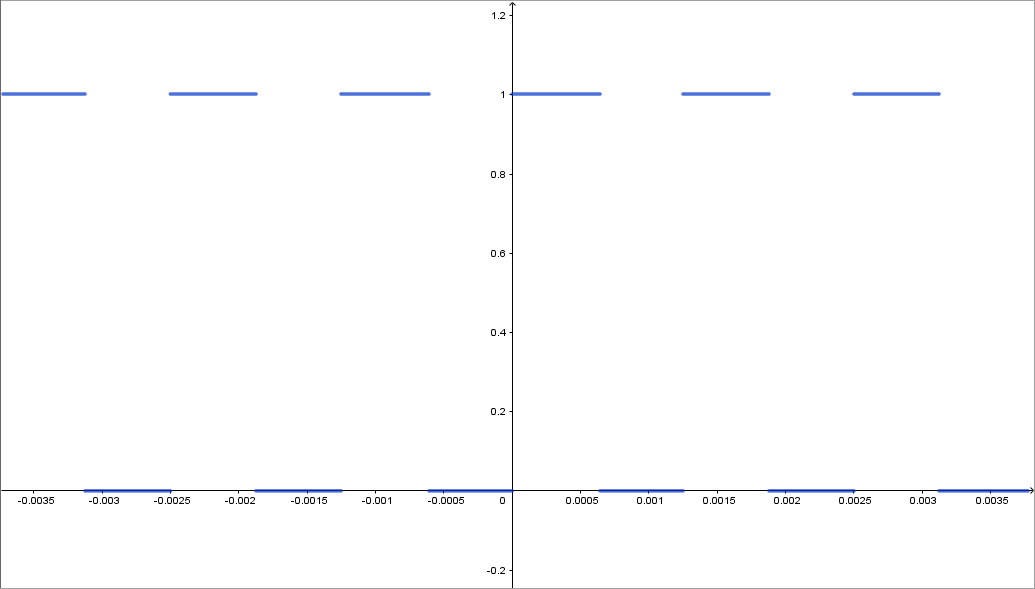
\includegraphics[width=.95\textwidth]{figuras/grafioflim.png}
    \caption{Gráfico de $f(t) =\frac{1}{2} + \frac{2}{\pi} \left( \sum\limits_{n = 0}^\infty \frac{\sen((2n+1) \omega_o t)}{2n+1} \right)  $}
    \label{figugraf}
\end{figure}
\newpage




Alguns exemplos clássicos de séries de Fourier são a \textbf{triangle wave} $\Lambda (x),$ a \textbf{sawtooth wave} $N(x)$ e a já citada \textbf{square wave} $\sqcap\ \hspace{-7pt}\sqcup (x):$

\[
\Lambda (x) = \cos(x) + \frac{\cos(3x)}{3^2} + + \frac{\cos(5x)}{5^2} + \frac{\cos(7x)}{7^2} + \frac{\cos(9x)}{9^2} + \ldots \]
\[
N(x) = \sen(x) + \frac{\sen(2x)}{2} + \frac{\sen(3x)}{3} + \frac{\sen(4x)}{4} + \frac{\sen(5x)}{5} + \ldots
\]
\[
\sqcap\ \hspace{-7pt}\sqcup (x) = \sen(x) + \frac{\sen(3x)}{3} + \frac{\sen(5x)}{5} + \frac{\sen(7x)}{7} + \frac{\sen(9x)}{9} + \ldots
\]


Vamos retornar à nossa série \ref{equa} e verificar que ela é de fato a série de Fourier de \ref{limite}:
\begin{equation}
f(t) = \left\{\begin{array}{lc}
1, & \mbox{se } t \in \bigcup\limits_{\ell =-\infty}^\infty \left] \frac{2 \ell \pi}{\omega_0}, \frac{(2 \ell + 1) \pi}{\omega_0} \right] \\
0, & \mbox{caso contrário.} 
\end{array} \right.
\end{equation}

Como visto, esta função admite uma série de Fourier\footnote{Não entraremos em questões sobre condições para existência da série de Fourier de uma dada função} da forma
\[
 c_0 + \sum\limits_{n = 1}^\infty a_n \cos(n \omega_0 t) + \sum\limits_{n = 1}^\infty b_n \sen(n \omega_0 t) 
\]
Pelo que sabemos de \ref{coefi}, temos que:
\[
c_0 =  \frac{1}{2 \pi} \int\limits_{-\pi}^\pi f(x) \dif {x} = \frac{1}{2 \pi}  \underbrace{\left(\int\limits_{-\pi}^{\frac{(1 - \omega_0) \pi}{\omega_0}} 1 \dif {x} + \int\limits_{\frac{(1 - \omega_0) \pi}{\omega_0}}^{\frac{(2 - \omega_0) \pi}{\omega_0}} 1 \dif {x} + \ldots + \int\limits_{\frac{(\omega_0 - 1) \pi}{\omega_0}}^{\pi} 1 \dif {x} \right)}_{\textcolor{blue}{\omega_0 \ \mbox{vezes} } }   = \]

\[
\frac{\textcolor{blue}{\omega_0}}{2 \pi} \left( \left( \frac{(1 - \omega_0) \pi}{\omega_0} + \pi \right) + \left( \frac{(2 - \omega_0) \pi}{\omega_0} - \frac{(1 - \omega_0) \pi}{\omega_0} \right) + \ldots +  \left( \pi - \frac{(\omega_0 - 1) \pi}{\omega_0}  \right)  \right) = 
\]
\[
\frac{\omega_0}{2 \pi} \cdot \frac{\pi}{\omega_0} = \frac{1}{2} \Rightarrow \boxed{c_0 = \frac{1}{2}}
\]
Usando que $\int\limits_a^b \cos(kx) \dif x = \frac{\sen(bk) - \sen(ak)}{k},$ temos $a_n=$
\[
\frac{1}{\pi} \underbrace{\left(\int\limits_{-\pi}^{\frac{(1 - \omega_0) \pi}{\omega_0}} 1\cdot \cos(n \omega_0 x) \dif {x} + \int\limits_{\frac{(1 - \omega_0) \pi}{\omega_0}}^{\frac{(2 - \omega_0) \pi}{\omega_0}} 1 \cdot\cos(n \omega_0 x) \dif {x} + \ldots + \int\limits_{\frac{(\omega_0 - 1) \pi}{\omega_0}}^{\pi} 1 \cdot \cos(n \omega_0 x) \dif {x} \right)}_{\textcolor{blue}{\omega_0 \ \mbox{vezes} } } =
\]
\[
\frac{\textcolor{blue}{\omega_0}}{\pi} \left( \frac{\sen\left(\frac{(1 - \omega_0) \pi}{\omega_0}  n \omega_0\right) - \sen\left(- \pi  n \omega_0\right)}{n \omega_0}  +  
\frac{\sen\left(\frac{(2 - \omega_0) \pi}{\omega_0}  n \omega_0\right) - \sen\left(\frac{(1 - \omega_0) \pi}{\omega_0}   n \omega_0\right)}{n \omega_0}  + \ldots \right.\]\[\left. + \frac{\sen\left(\pi  n \omega_0\right) - \sen\left(\frac{(\omega_0 - 1) \pi}{\omega_0}   n \omega_0\right)}{n \omega_0}    \right) =
\frac{\omega_0}{\pi} \left( \frac{ \cancel{\sen\left(n(1 - \omega_0) \pi \right)} + \sen\left( \pi  n \omega_0\right)}{n \omega_0}  +  \right.\]\[ \left.
\frac{\bcancel{\sen\left(  n(2 - \omega_0) \pi \right)} - \cancel{\sen\left(n(1 - \omega_0) \pi\right)}}{n \omega_0}  + \ldots + \frac{\sen\left(\pi  n \omega_0\right) - \xcancel{\sen\left(n(\omega_0 - 1) \pi  \right)}}{n \omega_0} \right) =
\]

\[
\frac{\textcolor{Laranja}{\omega_0}}{\pi} \left( \frac{\sen( \pi n \omega_0) + \sen( \pi n \omega_0) }{n \textcolor{Laranja}{\omega_0} } \right) = \frac{2}{\pi} \left(\frac{1}{n} \sen( \pi n \omega_0)\right) \Rightarrow \boxed{ a_n = \frac{2}{\pi} \left(\frac{1}{n} \sen( \pi n \omega_0)\right) }
\]


Analogamente ao feito acima, usando que $\int\limits_a^b \cos(kx) \dif x = \frac{\cos(bk) - \cos(ak)}{k},$ temos $b_n=$
\[
\frac{1}{\pi} \underbrace{\left(\int\limits_{-\pi}^{\frac{(1 - \omega_0) \pi}{\omega_0}} 1\cdot \sen(n \omega_0 x) \dif {x} + \int\limits_{\frac{(1 - \omega_0) \pi}{\omega_0}}^{\frac{(2 - \omega_0) \pi}{\omega_0}} 1 \cdot\sen(n \omega_0 x) \dif {x} + \ldots + \int\limits_{\frac{(\omega_0 - 1) \pi}{\omega_0}}^{\pi} 1 \cdot \sen(n \omega_0 x) \dif {x} \right)}_{\textcolor{blue}{\omega_0 \ \mbox{vezes} } } =
\]
\[
\frac{\textcolor{blue}{\omega_0}}{\pi} \left( \frac{\cos\left(\frac{(1 - \omega_0) \pi}{\omega_0}  n \omega_0\right) - \cos\left(- \pi  n \omega_0\right)}{n \omega_0}  +  
\frac{\cos\left(\frac{(2 - \omega_0) \pi}{\omega_0}  n \omega_0\right) - \cos\left(\frac{(1 - \omega_0) \pi}{\omega_0}   n \omega_0\right)}{n \omega_0}  + \ldots \right.\]\[\left. + \frac{\cos\left(\pi  n \omega_0\right) - \cos\left(\frac{(\omega_0 - 1) \pi}{\omega_0}   n \omega_0\right)}{n \omega_0}    \right) =
\frac{\omega_0}{\pi} \left( \frac{ \cancel{\cos\left(n(1 - \omega_0) \pi \right)} - \cos\left(- \pi  n \omega_0\right)}{n \omega_0}  +  \right.\]\[ \left.
\frac{\bcancel{\cos\left(  n(2 - \omega_0) \pi \right)} - \cancel{\cos\left(n(1 - \omega_0) \pi\right)}}{n \omega_0}  + \ldots + \frac{\cos\left(\pi  n \omega_0\right) - \xcancel{\cos\left(n(\omega_0 - 1) \pi \right) }}{n \omega_0} \right) =
\]
\[
\frac{\omega_0}{\pi} \left(\frac{\cos( \pi n \omega_0) - \cos( \pi n \omega_0)}{n \omega_0} \right) = 0 \Rightarrow \boxed{b_n = 0}
\]

Utilizando os coeficientes de Fourier encontrados, temos que
\[
\textcolor{violet}{c_0} + \sum\limits_{n = 1}^\infty \textcolor{Verde}{a_n} \cos(n \omega_0 t) + \sum\limits_{n = 1}^\infty \textcolor{Rosa}{b_n} \sen(n \omega_0 t)  =
\]
\[
\textcolor{violet}{\frac{1}{2}} + \sum\limits_{n = 1}^\infty \textcolor{Verde}{\frac{2}{\pi} \left(\frac{1}{n} \sen( \pi n \omega_0)\right) } \cos(n \omega_0 t) + \sum\limits_{n = 1}^\infty \textcolor{Rosa}{0} \cdot \sen(n \omega_0 t)  = 
\]
\[
\frac{1}{2} + \frac{2}{\pi} \sum\limits_{n = 1}^\infty \frac{1}{n} \left( \sen( \pi n \omega_0) \cos(n \omega_0 t) \right) =
\]
\[
\frac{1}{2} + \frac{2}{\pi} \sum\limits_{n = 1}^\infty \frac{1}{2n}  \sen( 2 \pi n \omega_0 t ) = \frac{1}{2} + \frac{2}{\pi} \sum\limits_{k = 0}^\infty \frac{\sen( (2k+1) \omega_0 t) }{2k+1},
\]
que é exatamente a série \ref{equa}.

Os gráficos mostram que é possível utilizar séries de Fourier para aproximar uma função que representa um sinal digital por meio de uma série infinita de senos e cossenos. As séries de senos são formas fundamentais do sinal analógico periódico. Logo, estamos realizando a conversão de um sinal analógico em um sinal digital.

Observe que, nos desenhos dos gráficos feitos nas figuras \ref{fig:1}, \ref{fig:2}, \ref{fig:3} e \ref{fig:4}, as figuras tendem ao gráfico do sinal digital, mas nos "picos de mudança" (saltos) dos sinais, ocorre uma pequena oscilação. Ou seja, a convergência das somas parciais da série de Fourier de uma função em torno de um salto apresenta oscilações cujas amplitudes não convergem para zero. A convergência ponto a ponto acontece, mas se olharmos para o valor absoluto da diferença entre a função e soma parcial sempre encontramos um ponto onde esse valor é maior do que a amplitude do salto. Esse fenômeno é chamado de \emph{Fenômeno de Gibbs}.


Vamos utilizar séries de Fourier para encontrar soluções para certos tipos de EDPs.


\section{Convergência em média quadrática}
Notemos que a série de Fourier de uma função periódica $f \colon \mathbb{R} \to \mathbb{R}$ de período $2 L$ está bem-definida se $\int\limits_{-L}^L | f(x) | \dif x < \infty.$
\begin{definicao}
Seja uma função periódica $f \colon \mathbb{R} \to \mathbb{R}$ de período $2 L$ e sua série de Fourier dada por
\[f(x) = \frac{A_0}{2} + \sum\limits_{k = 1}^\infty A_k \cos \left( \frac{k \pi x}{L} \right) \sum\limits_{k = 1}^\infty B_k \sen \left( \frac{k \pi x}{L} \right)\]
Então, dizemos que 
\[
s_n(x) = \frac{A_0}{2} + \sum\limits_{k = 1}^n A_k \cos \left( \frac{k \pi x}{L} \right) \sum\limits_{k = 1}^n B_k \sen \left( \frac{k \pi x}{L} \right)
\]
é a $n$-ésima \emph{soma parcial} da série.
\end{definicao}
\begin{teorema}
Se $\int\limits_{-L}^{L} f^2 (x) \dif x < \infty,$ então
\[
\lim\limits_{n \to \infty} \int\limits_{-L}^{L} (s_n(x) - f(x))^2 \dif x = 0.
\]

\end{teorema}

\begin{teorema}
Se $f \colon \mathbb{R} \to \mathbb{R}$ é periódica, e é $\mathcal{C}^1,$ então $s_n \to f$ uniformemente.
\end{teorema}

\begin{definicao}
Seja $f \colon \mathbb{R} \to \mathbb{R}$ uma função periódica de período $2L.$ Dizemos que $f$ é $\mathcal{C}^1$ por trechos se $f \in \mathcal{C}^1$ exceto numa quantidade finita de pontos, e nesses pontos os limites laterais de $f$ e $f^\prime$ existem.
\end{definicao}

\begin{teorema}[Teorema de Fejér]
Se $f$ é $\mathcal{C}^1$ por trechos então para todo $x \in [-L, L],$ temos que
\[
s_n \to \frac{f(x^{+}) + f(x^{-1})}{2}
\]
Em particular, $s_n \to f$ nos pontos em que $f$ é contínua.
\end{teorema}
\begin{proof}
Temos que
\[
s_n(x) = \frac{1}{2 \pi} \int\limits_{- \pi}^\pi + \frac{1}{\pi} \sum\limits_{k = 1}^n \cos k x \left(  \int\limits_{- \pi}^\pi f(y) \cos ky \dif y \right) + \sen k x \left(  \int\limits_{- \pi}^\pi f(y) \sen ky \dif y \right) =
\]
\[
\frac{1}{2 \pi} \int\limits_{- \pi}^{\pi} \left(  1 + 2 \sum\limits_{k = 1}^n \textcolor{red}{( \cos kx \cos ky + \sen kx \sen k y)} \right) f(y) \dif y =
\]
\[
\frac{1}{2 \pi} \int\limits_{- \pi}^{\pi} \left(  1 + 2 \sum\limits_{k = 1}^n \textcolor{red}{\cos k(x-y)}\right) f(y) \dif y
\]
\end{proof}


\begin{exemplo}
Seja $f(x)$ uma função periódica de período $2 \pi$ tal que $f(x) = \abs{x}$ para $x \in [-\pi, \pi].$ Temos:
\[
A_0 = \frac{1}{\pi} \int\limits_{- \pi}^\pi \abs{x} \dif x = \frac{2}{\pi} \int\limits_{0}^\pi = x \dif x = \pi
\]
\[
A_k = \frac{1}{\pi} \int\limits_{-\pi}^{\pi} \abs{x} \cos(mx) \dif x = \frac{2}{\pi} \int\limits_0^\pi x \cos (mx) \dif x = \frac{2}{\pi} \left( \frac{\sen(mx)}{x} \Bigg|_0^\pi - \frac{2}{\pi} \int\limits_0^\pi \frac{\sen(mx)}{x} \dif x \right) = \]\[0 + \frac{2}{\pi m} \frac{\cos(mx)}{x} \Bigg|_0^\pi = \frac{2}{\pi m^2} ((-1)^m  - 1)
\]
\[
B_k = \frac{1}{\pi} \int\limits_{-\pi}^{\pi} \abs{x} \sen(mx) \dif x = 0
\]
Ou seja, a série de Fourier de $f(x)$ é
\[
f(x) = \frac{\pi}{2} - \frac{4}{\pi} \left( \sum\limits_{m = 0}^\infty \frac{\cos((2m+1)x)}{(2m+1)^2}\right) = \frac{\pi}{2} - \frac{4}{\pi} \left(   \cos(x) + \frac{\cos(3x)}{3^2} + + \frac{\cos(5x)}{5^2} + \frac{\cos(7x)}{7^2} + \ldots  \right) = \]\[ \frac{\pi}{2} - \frac{4}{\pi}\Lambda (x)
\]

Como $f$ é $\mathcal{C}^1$ por trechos, então o teorema de Fejér se aplica. Além disso, $f$ é contínua, o que nos permite escrever
\[
\abs{x} = \frac{\pi}{2} - \frac{4}{\pi} \left( \sum\limits_{m = 0}^\infty \frac{\cos((2m+1)x)}{(2m+1)^2}\right), \mbox{para } -\pi \le x \le \pi.
\]
Tomando $k = 0,$ obtemos que
\[0 = \frac{\pi}{2} - \frac{4}{\pi} \left( \textcolor{Floresta}{1 + \frac{1}{9} + \frac{1}{25} + \ldots }\right) \Rightarrow \frac{\pi}{2} = \frac{4}{\pi} \textcolor{Floresta}{\sum\limits_{k = 1}^\infty \frac{1}{(2k-1)^2}} \Rightarrow \boxed{\sum\limits_{k = 1}^\infty \frac{1}{(2k-1)^2} = \frac{\pi^2}{8}}
\]
\end{exemplo}

\begin{exemplo}
Vamos utilizar a série \ref{equa}, para $\omega_0 = \pi.$ Sendo
\[
g(x) = \begin{array}{cc}
    0 & \mbox{se} -1 < x < 0  \\
    1  & \mbox{se} 0 < x < 1
\end{array}
\]
Como $g(x)$ é $\mathcal{C}^1$ por trechos, temos que
\[
1 = \frac{1}{2} + \frac{2}{\pi} \left(\sen(\pi x) + \frac{\sen(3 \pi x)}{3} + \frac{\sen(5 \pi x)}{5}  + \ldots \right), \mbox{para } 0< x < 1
\]
\[
0 = \frac{1}{2} + \frac{2}{\pi} \left(\sen(\pi x) + \frac{\sen(3 \pi x)}{3} + \frac{\sen(5 \pi x)}{5}  + \ldots \right), \mbox{para } -1< x <0
\]
pois $g(x)$ é contínua em $(-1, 0)$ e em $(0, 1)$. Porém no ponto $0$, a série não se aproxima de $g (0)$ mas sim de
\[
\frac{g(0^+) + g(0^{-}}{2} = \frac{1}{2}
\]
o que pode ser confirmado substituindo $x = 0$ na série de Fourier. Por outro lado, tomando $x = \frac{1}{2},$ obtemos
\[1 = \frac{1}{2} + \frac{2}{\pi} \left(1- \frac{1}{3} + \frac{1}{5}  - \frac{1}{7} + \ldots \right) \Rightarrow \boxed{\sum\limits_{k = 1}^\infty \frac{(-1)^{k+1}}{(2k-1)} = \frac{\pi}{4}}
\]
\end{exemplo}

\begin{teorema}[Parseval]
Temos que
\[
\int\limits_{- L}^L f(x)^2 \dif x = \frac{A_0^2}{2} + \sum\limits_{n = 1}^\infty (A_n^2 + B_n^2)
\]
\end{teorema}

\section{Equação de Laplace}
\begin{definicao}
Uma função é harmônica se $\Delta u = 0.$
\end{definicao}

\end{document}


















Sejam $K[F(X)]$  anel de grupo livre e $K \alngle \langle X \rangle \rangle$ o anel das séries formais com coeficientes em K. Seja $\vartheta$ uma relação de comutação parcial em $X.$
Definimos em $K[F(X)]$ a derivação dada por
\[
\partial_{x_i} (x_j) = \frac{\partial x_i}{\partial x_j} = \delta_{ij}
\]
e definimos a derivação em várias variáveis por:
\[\frac{\partial f}{\partial x_{i_1} x_{i_2} \ldots x_{i_n} } = \frac{\partial }{\partial x_{i_1}} \frac{\partial f}{\partial x_{i_2} \ldots x_{i_n}}\]

Considere 
\[\fullfunction{\psi}{K[F(X)]}{K\langle \langle X \rangle \rangle}{f}{\psi(f) = \sum \varepsilon\left( \frac{\partial f}{\partial x_i \ldots x_j} \right)x_i \ldots x_j}
\]
$\psi$é injetora. Sejam $\varphi$ e $\tilde{\varphi}$ as imersões $\varphi(x) = \overline{x}.$ Podemos então considerar
\[\fullfunction{\psi}{K[F(X\vartheta)]}{K\langle \langle X, \vartheta \rangle \rangle}{f}{\psi(f) = \sum \varepsilon\left( \varphi \left(\frac{\partial f}{\partial x_i \ldots x_j} \right) \right) \overline{x_i \ldots x_j}}
\]
Então, $\tilde{\psi}$ é injetora?

Queremos mostrar que $\tilde{\psi}(\overline{f}) = f \Rightarrow\overline{f}= 0.$ Para isso, é suficiente ver que $\ker \varphi = \ker \tilde{\varphi}?$










